\uuid{mH1D}
\chapitre{Fonction de plusieurs variables}
\niveau{L2}
\module{Analyse}
\sousChapitre{Surface représentative}
\titre{Fonction de deux variables et surface représentative}
\theme{fonctions de plusieurs variables}
\auteur{}
\datecreate{2023-02-23}
\organisation{AMSCC}
\difficulte{}
\contenu{
	
	A chaque fonction définie ci-dessous (1-6), associer sa surface représentative (A-F).
	
	\begin{multicols}{3}
		\begin{enumerate}
			\item $f(x,y) = |x|+|y|$
			\item $f(x,y) = |xy|$
			\item $f(x,y) = \frac{1}{1+x^2+y^2}$
			\item $f(x,y) = (x^2-y^2)^2$
			\item $f(x,y) = (x-y)^2$
			\item $f(x,y) = \sin(|x|+|y|)$
		\end{enumerate}
	\end{multicols}
	
	\begin{minipage}{0.5\textwidth}
		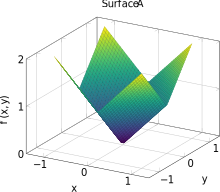
\includegraphics[]{pdf/mH1D-tikz-1}
	\end{minipage}
	\hfill
	\begin{minipage}{0.5\textwidth}
		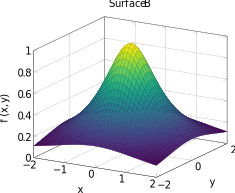
\includegraphics[]{pdf/mH1D-tikz-2}
	\end{minipage}
	
	\begin{minipage}{0.5\textwidth}
		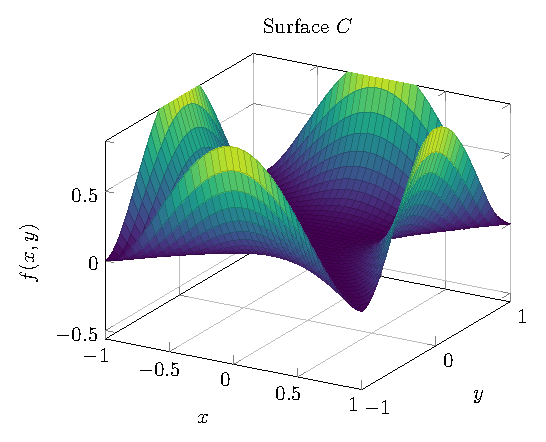
\includegraphics[]{pdf/mH1D-tikz-3}
	\end{minipage}
	\hfill
	\begin{minipage}{0.5\textwidth}
		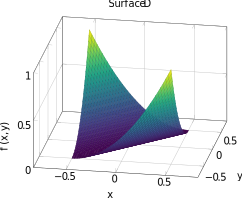
\includegraphics[]{pdf/mH1D-tikz-4}
	\end{minipage}
	
	\begin{minipage}{0.5\textwidth}
		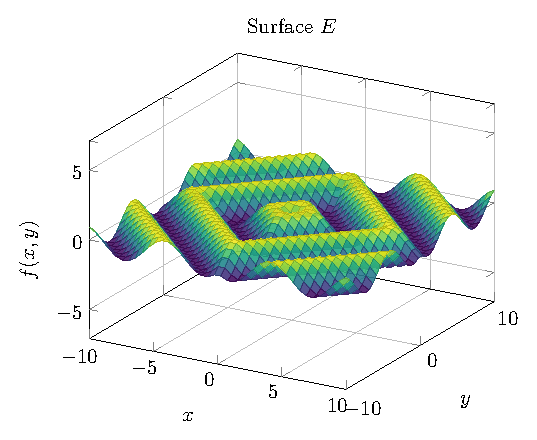
\includegraphics[]{pdf/mH1D-tikz-5}
	\end{minipage}
	\hfill
	\begin{minipage}{0.5\textwidth}
		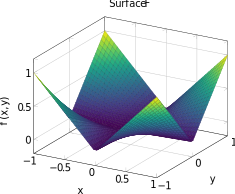
\includegraphics[]{pdf/mH1D-tikz-6}
\end{minipage}}
